\documentclass[12pt]{article}
%For use url link
\usepackage{hyperref}
%For use color
\usepackage[dvipsnames]{xcolor}
%Import geometry for smaller top
\usepackage{geometry}
% Required for inserting images
\usepackage{graphicx}
\graphicspath{{./images/}}
%Header and footer
\usepackage{fancyhdr}
%Language setting
\usepackage[utf8]{inputenc}
\usepackage[T2A]{fontenc}
\usepackage[russian]{babel}

\hypersetup{
    colorlinks=true,
    linkcolor=blue,
    filecolor=magenta,      
    urlcolor=cyan,
    pdftitle={Overleaf Example},
    pdfpagemode=FullScreen,
}

\urlstyle{same}

\geometry{a4paper,
 total={170mm,257mm},
 left=20mm,
 top=30mm,
 bottom=25mm,
 }

\fancypagestyle{first style}
{
\chead{\footnotesize{Санкт-Петербургский Национальный Исследовательский Университет ИТМО\\Факультет Программной Инженерии и Компьютерной Техники}}
\cfoot{\footnotesize{Санкт-Петербург 2023г.}}
\renewcommand{\headrulewidth}{0pt}
}

\begin{document}

\pagestyle{fancy}
$\thispagestyle{first style}$

\centering{
\includegraphics[scale=0.5]{LogoITMO}}

\vspace{25mm}

\centering{Вариант №373342\\Лабораторная работа№1\\По дисциплине\\Веб-программирование}

\vspace{50mm}

\begin{flushright}
Выполнил студент группы P3215:\\Хромов Даниил Тимофеевич\\
\vspace{5mm}
Преподаватель:\\Кустарев Максим Андреевич\\
\end{flushright}

\newpage

\pagestyle{empty}

\Large\textcolor{NavyBlue}{Задание}\\
\rmfamily\small
\vspace{5mm}
\raggedright
Разработать PHP-скрипт, определяющий попадание точки на координатной плоскости в заданную
область, и создать HTML-страницу, которая формирует данные для отправки их на обработку
этому скрипту.\\
\vspace{5mm}
Параметр R и координаты точки должны передаваться скрипту посредством HTTP-запроса.
Скрипт должен выполнять валидацию данных и возвращать HTML-страницу с таблицей,
содержащей полученные параметры и результат вычислений - факт попадания или непопадания
точки в область. Предыдущие результаты должны сохраняться между запросами и отображаться в
таблице.\\
\vspace{5mm}
Кроме того, ответ должен содержать данные о текущем времени и времени работы скрипта.\\
\vspace{5mm}

\textbf{Разработанная HTML-страница должна удовлетворять следующим требованиям:}\\
\begin{itemize}
    \item Для расположения текстовых и графических элементов необходимо использовать
    табличную верстку.\\
    \item Данные формы должны передаваться на обработку посредством GET-запроса.\\
    \item Таблицы стилей должны располагаться в отдельных файлах.\\
    \item При работе с CSS должно быть продемонстрировано использование селекторов дочерних
    элементов, селекторов элементов, селекторов потомств, селекторов псевдоклассов а также
    такие свойства стилей CSS, как наследование и каскадирование.\\
    \item HTML-страница должна иметь "шапку", содержащую ФИО студента, номер группы и
    номер варианта. При оформлении шапки необходимо явным образом задать шрифт
    (fantasy), его цвет и размер в каскадной таблице стилей.\\
    \item Отступы элементов ввода должны задаваться в пикселях.\\
    \item Страница должна содержать сценарий на языке JavaScript, осуществляющий валидацию
    значений, вводимых пользователем в поля формы. Любые некорректные значения
    (например, буквы в координатах точки или отрицательный радиус) должны блокироваться.\\
\end{itemize}

\vspace{1cm}

\centering{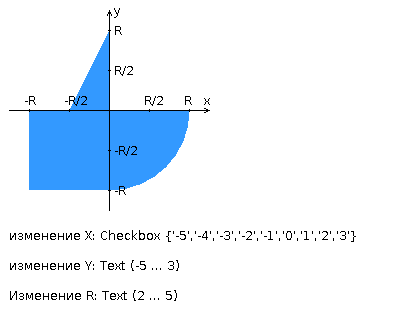
\includegraphics[scale=0.8]{SvgImage}}

\newpage

\Large\textcolor{NavyBlue}{Вывод по работе}\\

\rmfamily\small
\vspace{5mm}
\raggedright
В результате выполнения лабораторной работы были получены навыки создания веб-
приложений: фронтенд на HTML, CSS, JavaScript; бэкенд на PHP. В процессе выполнения я
получил представление о архитектуре клиент-сервер и протоколе HTTP для передачи данных.
Узнал про две концепции веб-разработки: REST и RPC. Наибольшей сложностью в разработке
оказался объём материала, который необходимо изучить.\\
\vspace{5mm}
Созданное веб-приложение доступно по адресу \url{https://se.ifmo.ru/~s373336/web/lab1/}.

\end{document}